% THIS TEMPLATE IS A WORK IN PROGRESS
% Adapted from an original template by faculty at Reykjavik University, Iceland

\documentclass{scrartcl}
\input{File_Setup.tex}
\usepackage[utf8]{inputenc}
\usepackage{graphicx,epsfig}
\usepackage{hyperref}
\usepackage{adjustbox}
\usepackage{multirow}
\usepackage{amsmath}
\usepackage{booktabs}
\usepackage{microtype}
\usepackage[inkscapelatex=false]{svg}
\usepackage{bbm}


\hypersetup{
   colorlinks   = true,                               %Colours links instead of ugly boxes
   urlcolor     = blue,                               %Colour for external hyper links
   linkcolor    = blue,                               %Colour of internal links
   citecolor    = red,                                %Colour of citations
   setpagesize  = false,
   linktocpage  = true,
}
\graphicspath{ {fig/} }



\renewenvironment{abstract}{
    \centering
    \textbf{Abstract}
    \vspace{0.5cm}
    \par\itshape
    \begin{minipage}{0.7\linewidth}}{\end{minipage}
    \noindent\ignorespaces
}
% ------------------------------------------------------------------------------------------------------------------------

\begin{document}
%Title of the report, name of coworkers and dates (of experiment and of report).
\begin{titlepage}
	\centering
	\includegraphics[width=0.6\textwidth]{GW_logo.eps}\par
	\vspace{2cm}
	%%%% COMMENT OUT irrelevant lines below: Data Science OR Computer Science OR none
	{\scshape\LARGE Data Science Program \par}
	\vspace{1cm}
	{\scshape\Large Capstone Report - Fall 2024\par}
	\vspace{1.5cm}
	{\huge\bfseries MyRAG - Advancing Retrieval-Augmented Generation with Comparative Analysis of Standard RAG, ColBERT Reranking, and RAPTOR Architectures \par}
	\vspace{2cm}
	%%%% AUTHOR(S)
	{\Large\itshape Meet Daxini \\}\par
	\vspace{1.5cm}
	supervised by\par
	%%%% SUPERVISOR(S)
	Amir Jafari
\newpage

	\vfill
	\begin{abstract}
Retrieval-Augmented Generation (RAG) has emerged as a powerful paradigm for providing personalized, relevant, and current information to user queries by combining large language models (LLMs) with external retrieval modules. This paper presents \textit{MyRAG}, an open-source system that unifies and compares different state-of-the-art RAG architectures and retrieval techniques. This paper explores embeddings, vector databases, and advanced retrieval methods, including ColBERT-based reranking and the hierarchical summarization-based RAPTOR architecture. By evaluating MyRAG on the BioASQ and Hugging Face Document QA datasets, demonstrates how different configurations impact retrieval accuracy and downstream QA performance. The results offer insights into optimizing RAG pipelines, guiding both practitioners and researchers toward more efficient and effective retrieval-augmented generation.
	\end{abstract}
	\vfill
% Bottom of the page
\end{titlepage}
\tableofcontents
\newpage
% ------------------------------------------------------------------------------------------------------------------------
\section{Introduction}

The exponential growth of digital information has increased the demand for intelligent systems that can efficiently retrieve relevant context and answer complex questions. Large Language Models (LLMs) often possess extensive parametric knowledge, but may lack reliable, up-to-date information. Retrieval-Augmented Generation (RAG) has gained prominence as a solution to this challenge, bridging large-scale language understanding with external retrieval components to produce more grounded and accurate responses \cite{lewis2020retrieval, guu2020realm}.

In RAG pipelines, the LLM accesses external knowledge sources, retrieving relevant documents or chunks to augment its prompt. This approach enhances the model’s factual accuracy, reduces hallucinations, and updates knowledge without retraining the entire model. As the sizes of the context window continue to expand \cite{liu2023lost}, it is increasingly practical to provide LLMs with larger and more diverse sets of the retrieved context.

\begin{figure}[h]
    \centering
    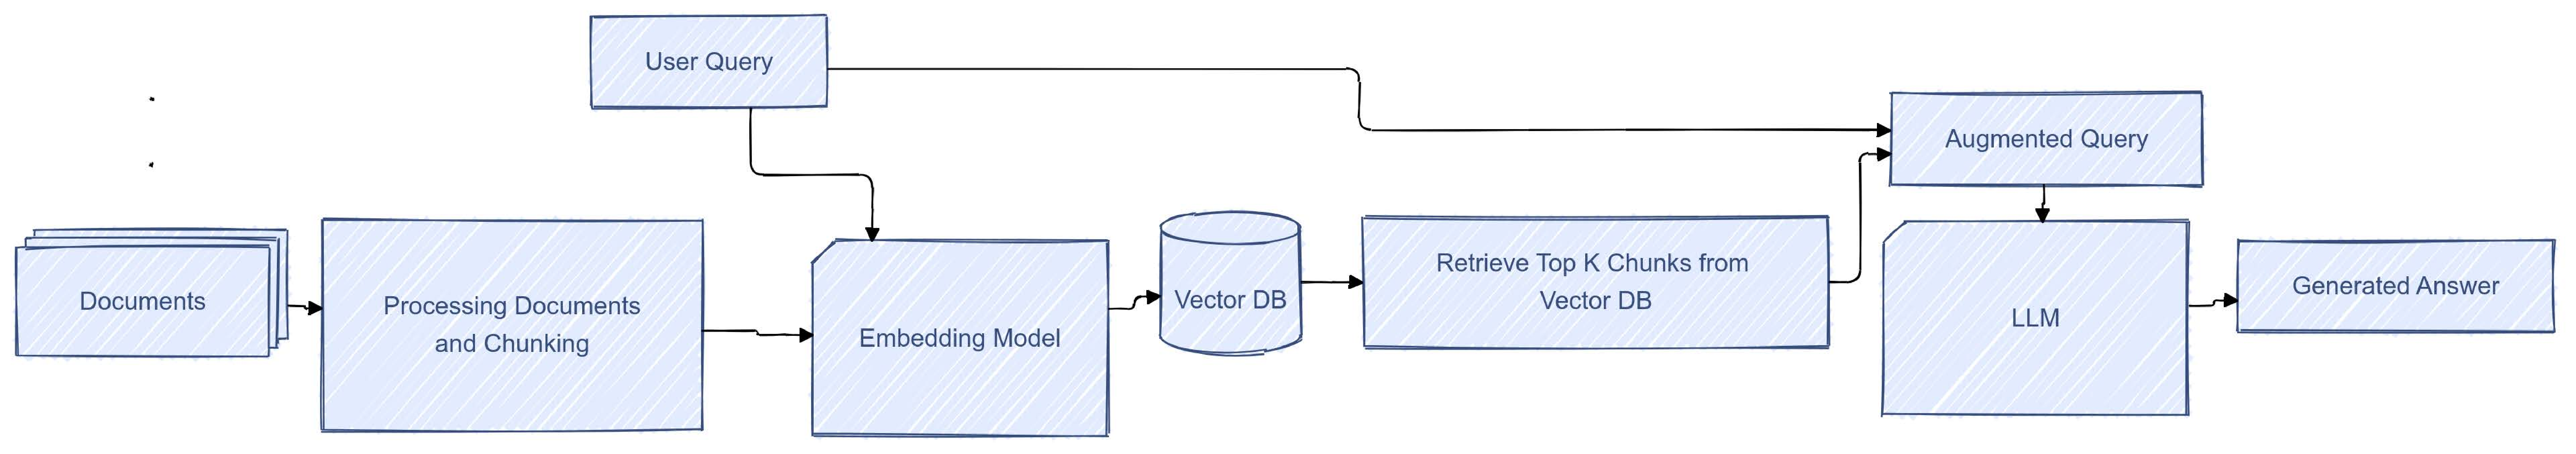
\includegraphics[width=\linewidth]{StandardRag.pdf} 
    \caption{Flow chart illustrating the standard RAG pipeline.}
    \label{fig:standard_rag_flow}
\end{figure}


Yet, not all retrieval pipelines are created equal. Various embedding models, vector databases, and advanced retrieval techniques can be combined to form a RAG system. For instance, This paper explores How Standard Rag with ColBERT \cite{khattab2020colbert} re-ranking can refine retrieved documents, while the RAPTOR architecture \cite{wu2021recursively, raptor2024} organizes and summarizes documents hierarchically. Understanding the trade-offs between these methods is key to building robust and scalable RAG systems.

This paper introduces \textit{MyRAG}, an open-source framework designed to compare multiple retrieval and augmented generation strategies systematically. We evaluate embeddings, vector stores, and advanced retrieval enhancements like ColBERT re-ranking and RAPTOR summarization, applying them on the BioASQ \cite{bioasq2023} and Hugging Face Document QA datasets \cite{huggingface2024docqa}. Our experiments aim to provide a clearer understanding of how these components influence retrieval accuracy and end-to-end QA performance.

%----------------- Problem Statement -----------------%
\section{Problem Statement}

While the Massive Text Embedding Benchmark (MTEB) \cite{muennighoff2022mteb} provides valuable insights into embedding model performance across diverse tasks, there remains a critical need for comprehensive evaluation of end-to-end RAG architectures. The current landscape lacks:

\begin{enumerate}
    \item \textbf{Architecture-Specific Evaluation:} Unlike MTEB's focus on embedding quality, MyRAG provides systematic comparison of different RAG architectures - ColBERT reranking \cite{khattab2020colbert}, and RAPTOR hierarchical retrieval \cite{wu2021recursively, raptor2024} - using consistent datasets, metrics, vector stores (Chroma and DeepLake) and quantization strategies.
    
    \item \textbf{Resource-Conscious Assessment:} MyRAG evaluates both 8-bit quantized and full-precision versions of popular embedding models addressing practical deployment considerations not covered by MTEB's leaderboard.
    
    \item \textbf{Intuitive Real-World Metrics:} MyRAG introduces straightforward measures beyond MTEB's technical metrics:
    \begin{itemize}
        \item Correct/Partial/Incorrect answer classification
        \item Multi-document per question retrieval accuracy 
        \item Response generation quality with context
        \item Resource utilization across architectures
    \end{itemize}
\end{enumerate}

Through this comprehensive evaluation framework, MyRAG helps practitioners select optimal combinations of embedding models (guided by MTEB's leaderboard), retrieval architectures, and implementation approaches. The framework supports both detailed technical assessment and simple, interpretable metrics that organizations need to optimize their RAG deployments across use cases and resource constraints. By offering comparison of standard RAG, ColBERT reranking, and RAPTOR approaches on multtiple datasets, MyRAG provides actionable insights for building more effective retrieval-augmented generation systems.


\textit{MyRAG} addresses this need by providing an open-source code framework that enables direct, end-to-end comparisons of RAG approaches. By incorporating multiple embedding models, vector databases (e.g., Chroma and DeepLake), reranking strategies (e.g., ColBERT), and hierarchical retrieval architectures (e.g., RAPTOR), \textit{MyRAG} provides a clear, cohesive platform for empirical evaluation. This approach ensures that even non-experts can understand performance trade-offs through accessible and practical metrics, ultimately guiding practitioners and researchers toward more optimal and tailored RAG solutions.
%----------------- MyRag System -----------------%
\section{MyRAG}
MyRAG builds on these works by offering a unified platform to compare multiple embeddings, vector stores, and retrieval strategies, including ColBERT and RAPTOR, on common benchmarks.
The MyRAG system provides a flexible pipeline to switch between embedding models, vector stores, and retrieval techniques. Key components include:

\subsection{Parsing Documents and Chunking}

\subsection{Embedding Models}

We integrate several embedding models:
\begin{itemize}
    \item NV-Embed-v2, Stella 1.5B, MXBai Large, Amazon Titan, all-MiniLM-L6-v2
\end{itemize}
These models differ in size, parameters, and performance trade-offs. We evaluate how embedding choice affects retrieval accuracy and QA outcomes.

\subsection{Vector Databases}

MyRAG supports Chroma and DeepLake, two vector databases optimized for similarity search with support for HNSW indices and cosine or L2 metrics. Initial experiments suggest that cosine similarity often performs better, though L2 metrics are also tested for completeness.

\subsection{ColBERT Reranking}


\begin{figure}[H]
	\centering
	\includegraphics[width=\linewidth]{Colbert.pdf}
	\caption{Flow chart of ColBert Reranking}
	\label{fig:colbert}
\end{figure}


\begin{figure}[H]
	\centering
	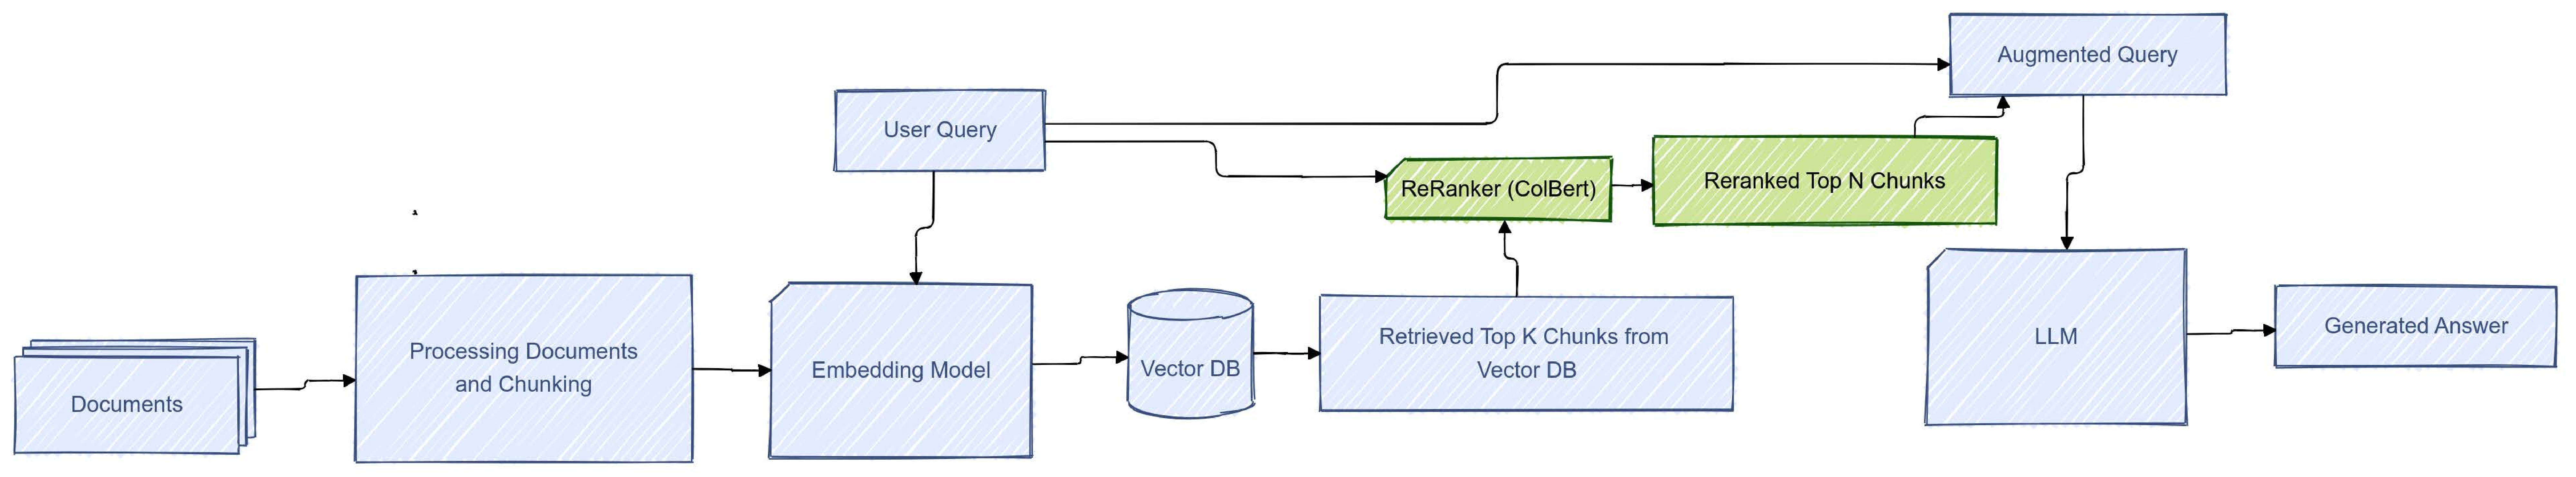
\includegraphics[width=\linewidth]{StandardRagWithReRanking.pdf}
	\caption{Flow chart of Standard Rag with ColBert Reranking as integrated in MyRag}
	\label{fig:reranking_rag}
\end{figure}

ColBERT \cite{khattab2020colbert} refines initial retrieval results by re-ranking passages based on fine-grained token-level similarities. This step often improves retrieval accuracy by ensuring that top-ranked documents are highly relevant to the query.

\subsection{RAPTOR}


\begin{figure}[H]
	\centering
	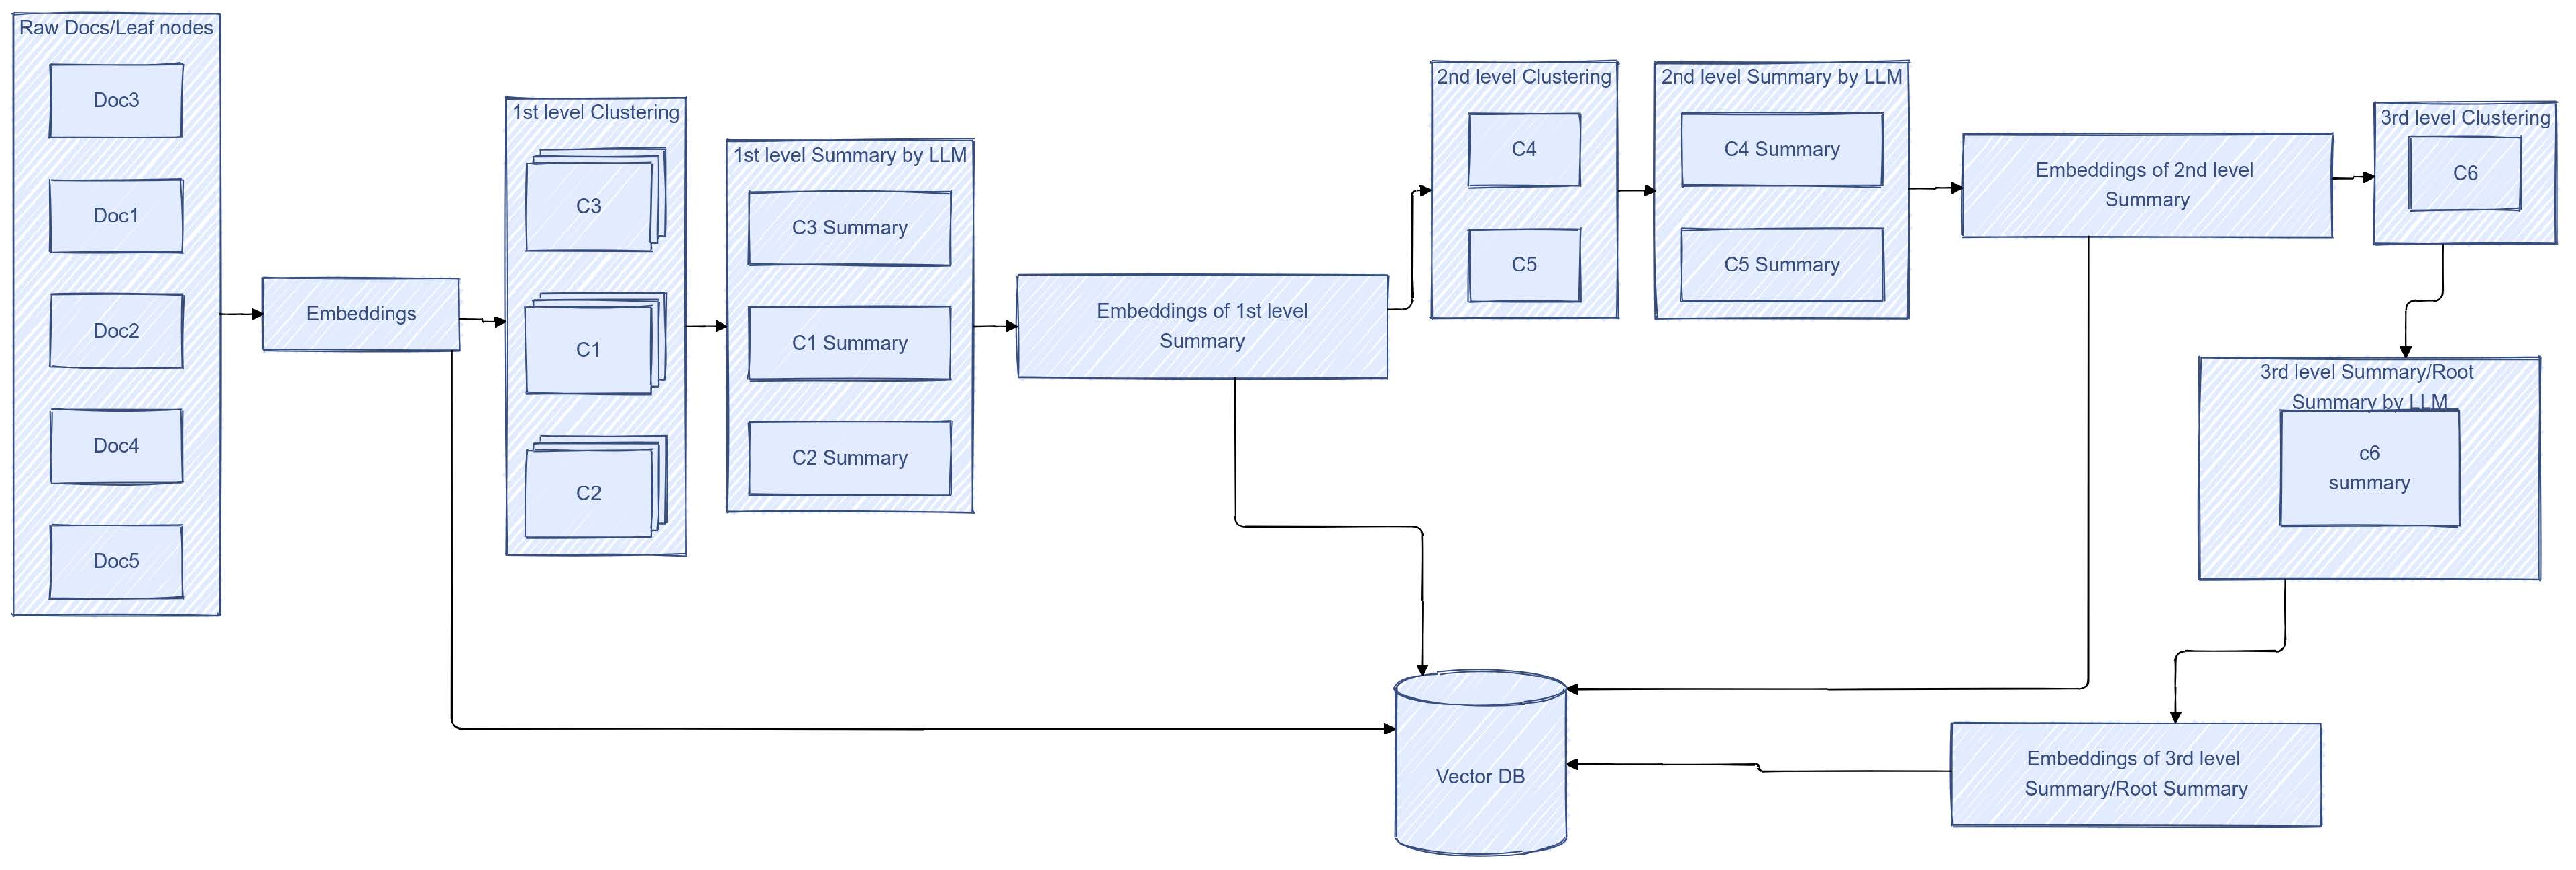
\includegraphics[width=\linewidth]{Raptor.pdf}
	\caption{Flow chart of RAPTOR Architecture as integrated in MyRAG}
	\label{fig:raptor}
\end{figure}

We incorporate RAPTOR \cite{wu2021recursively, raptor2024}, which uses hierarchical summarization to structure large corpora. RAPTOR builds a tree of summaries at increasing levels of abstraction. This architecture allows retrieval at multiple scales—broad thematic overviews down to granular details—enhancing multi-hop QA and reducing context fragmentation.

\subsection{Demo GUI}

%----------------- Evaluations and Results -----------------%
\section{Evaluations and Results}

%----------------- Datasets -----------------%
\subsection{Datasets}

\textbf{1. Hugging Face Document QA Evaluation Dataset:}

The \textit{huggingface\_doc\_qa\_eval} dataset is a synthetic dataset consisting of question-answer pairs extracted from the markdown files of the Hugging Face repository on GitHub. It is specifically designed for evaluating Retrieval-Augmented Generation (RAG) systems \cite{huggingface2024docqa}. The dataset contains a total of 65 unique questions, each paired with its corresponding answer, context, and source document path.

Out of the ten available columns in the dataset, the following four were used for evaluation:
\begin{itemize}
    \item \textbf{Context:} The content retrieved from the corresponding markdown file.
    \item \textbf{Question:} The query posed to the system.
    \item \textbf{Answer:} The ideal answer to the question.
    \item \textbf{Source\_doc:} The path to the markdown file in the Hugging Face GitHub repository.
\end{itemize}

The dataset was loaded in Parquet format using the Hugging Face API. Each question-answer pair was derived from a unique markdown file, ensuring there was no overlap in the source documents. This design allows for precise evaluation of RAG systems in retrieving relevant content from specific documents.

\textbf{2. BioASQ11 Challenge Dataset:}

The \textit{BioASQ11} dataset was obtained from the 2023 iteration of the BioASQ challenge, specifically Task Set B for biomedical question answering \cite{bioasq2023}. The training set (11b) consists of a total of 4,719 questions, each provided with gold-standard annotations, including concepts, article URLs, snippets, RDF triples, "exact" answers, and "ideal" answers.

Due to the size of the dataset and restrictions on accessing articles from certain URLs, a filtering process was applied:
\begin{itemize}
    \item Articles that required special accounts or credentials for access were excluded.
    \item To comply with server limitations on large-scale downloads, only a subset of 13 questions with 42 associated PDFs was retained for the evaluation.
\end{itemize}

For each retained question, answers are derived from 1 to 7 different PDFs. To facilitate evaluation, a CSV file was created on GitHub with the following columns:
\begin{itemize}
    \item \textbf{Question ID:} A unique identifier for each question.
    \item \textbf{Question:} The query posed.
    \item \textbf{Ideal Answer:} The gold-standard answer for the question.
    \item \textbf{Download Link:} The URL for downloading the article PDF.
    \item \textbf{PDF Reference:} The specific reference to the PDFs used for the answer.
\end{itemize}

A web scraping script was developed to retrieve PDF file URLs from the provided article links. This processed dataset enables systematic evaluation of retrieval accuracy and relevance in biomedical contexts.


\subsection{TOP-K Retrieval Accuracies}

To evaluate retrieval performance, we measure the accuracy of the top-\(k\) retrieved documents against the known relevant set of documents. For each query \(i\), let \(\text{retrieved}_i@k\) denote the set of top-\(k\) retrieved documents and \(\text{relevant}_i\) denote the set of all relevant documents. The top-\(k\) retrieval accuracy, \(\text{Accuracy@k}\), is calculated as:

\begin{equation}
\text{Accuracy@k} = \frac{1}{N} \sum_{i=1}^{N} 
    \begin{cases}
      \mathbbm{1}(\exists d \in \text{retrieved}_i@k : d \in \text{relevant}_i), & \text{if } |\text{relevant}_i| = 1 \text{ or } k = 1 \\[6pt]
      \frac{|\text{retrieved}_i@k \cap \text{relevant}_i|}{\min(k, |\text{relevant}_i|)}, & \text{otherwise}
    \end{cases}
\end{equation}

Here:
\begin{itemize}
    \item \(N\) is the total number of queries.
    \item \(\text{retrieved}_i@k\) are the top-\(k\) retrieved documents for the \(i\)-th query.
    \item \(\text{relevant}_i\) are the relevant documents for the \(i\)-th query.
    \item \(\mathbbm{1}\) is the indicator function that equals 1 if the condition is true and 0 otherwise.
\end{itemize}


\begin{table}[H]
\centering
\small
\begin{tabular}{l l c c c c c c c c}
\hline
\textbf{Model} & \textbf{Dataset} & \textbf{k=1} & \textbf{k=2} & \textbf{k=3} & \textbf{k=4} & \textbf{k=5} & \textbf{k=7} & \textbf{k=8} & \textbf{k=10} \\
\hline
\multirow{2}{*}{\texttt{NV-Embed-v2 (8-bit)}} 
 & BioASQ & 1.00 & 0.85 & 0.79 & 0.76 & 0.77 & 0.79 & 0.80 & 0.80 \\
 & HF QA  & 0.91 & 0.94 & 0.98 & 0.98 & 0.98 & 1.00 & 1.00 & 1.00 \\
\hline
\multirow{2}{*}{\texttt{all-MiniLM-L6-v2}} 
 & BioASQ & 0.62 & 0.58 & 0.51 & 0.47 & 0.57 & 0.54 & 0.57 & 0.61 \\
 & HF QA  & 0.58 & 0.66 & 0.72 & 0.74 & 0.77 & 0.80 & 0.82 & 0.83 \\
\hline
\multirow{2}{*}{\texttt{mxbai-embed-large-v1}} 
 & BioASQ & 1.00 & 0.92 & 0.77 & 0.70 & 0.74 & 0.77 & 0.79 & 0.79 \\
 & HF QA  & 0.95 & 0.95 & 0.95 & 0.95 & 0.95 & 0.98 & 0.98 & 0.98 \\
\hline
\multirow{2}{*}{\texttt{stella\_en\_1.5B\_v5}} 
 & BioASQ & 1.00 & 0.73 & 0.72 & 0.71 & 0.72 & 0.74 & 0.75 & 0.79 \\
 & HF QA  & 0.95 & 0.98 & 0.98 & 0.98 & 1.00 & 1.00 & 1.00 & 1.00 \\
\hline
\multirow{2}{*}{\texttt{stella\_en\_1.5B\_v5 (8-bit)}} 
 & BioASQ & 0.31 & 0.42 & 0.64 & 0.66 & 0.68 & 0.74 & 0.74 & 0.78 \\
 & HF QA  & 0.88 & 0.91 & 0.91 & 0.91 & 0.92 & 0.94 & 0.94 & 0.94 \\
\hline
\multirow{2}{*}{\texttt{titan-embed-text-v2}} 
 & BioASQ & 1.00 & 0.81 & 0.69 & 0.67 & 0.69 & 0.67 & 0.68 & 0.73 \\
 & HF QA  & 0.89 & 0.91 & 0.95 & 0.97 & 0.98 & 0.98 & 0.98 & 0.98 \\
\hline
\end{tabular}
\caption{Top-k Retrieval Accuracy Comparison of Embedding Models in Standard Rag}
\label{table:top_k_retrieval_accuracy_table}
\end{table}

As illustrated in Table  \ref{table:top_k_retrieval_accuracy_table}, the \texttt{NV-Embed-v2 (8-bit)} model, which utilizes 7.44 GB of GPU memory, performs comparably to the \texttt{stella\_en\_1.5B\_v5} model that consumes 9.25 GB. However, \texttt{stella\_en\_1.5B\_v5} achieves slightly better scores overall. Notably, the lightweight \texttt{mxbai-embed-large-v1}, which requires only 1.25 GB of GPU memory, performs equally well and, in some cases, even slightly better than \texttt{stella\_en\_1.5B\_v5}. While the \texttt{all-MiniLM-L6-v2} is also very lightweight, it does not perform as well. Additionally, the closed-source \texttt{titan-embed-text-v2} model from Amazon, does not outperform the open-source models. Parameters used while retrieval in appendix



\begin{table}[H]
\centering
\small
\begin{tabular}{l l c c c c c c c c}
\hline
\textbf{Model} & \textbf{Dataset} & \textbf{k=1} & \textbf{k=2} & \textbf{k=3} & \textbf{k=4} & \textbf{k=5} & \textbf{k=7} & \textbf{k=8} & \textbf{k=10} \\
\hline
\multirow{2}{*}{\texttt{NV-Embed-v2 (8-bit)}} 
 & BioASQ & 1.00 & 0.81 & 0.74 & 0.77 & 0.78 & 0.80 & 0.80 & 0.82 \\
 & HF QA  & 0.97 & 0.98 & 0.98 & 0.98 & 0.98 & 0.98 & 1.00 & 1.00 \\
\hline
\multirow{2}{*}{\texttt{all-MiniLM-L6-v2}} 
 & BioASQ & 0.85 & 0.77 & 0.72 & 0.67 & 0.69 & 0.72 & 0.72 & 0.73 \\
 & HF QA  & 0.88 & 0.89 & 0.89 & 0.89 & 0.91 & 0.91 & 0.91 & 0.91 \\
\hline
\multirow{2}{*}{\texttt{mxbai-embed-large-v1}} 
 & BioASQ & 1.00 & 0.88 & 0.77 & 0.73 & 0.74 & 0.80 & 0.82 & 0.82 \\
 & HF QA  & 0.92 & 0.97 & 0.97 & 0.98 & 0.98 & 0.98 & 0.98 & 0.98 \\
\hline
\multirow{2}{*}{\texttt{stella\_en\_1.5B\_v5}} 
 & BioASQ & 1.00 & 0.85 & 0.72 & 0.67 & 0.73 & 0.79 & 0.79 & 0.79 \\
 & HF QA  & 0.95 & 0.98 & 0.98 & 0.98 & 0.98 & 0.98 & 0.98 & 1.00 \\
\hline
\multirow{2}{*}{\texttt{stella\_en\_1.5B\_v5 (8-bit)}} 
 & BioASQ & 0.92 & 0.81 & 0.72 & 0.67 & 0.68 & 0.69 & 0.70 & 0.72 \\
 & HF QA  & 0.77 & 0.77 & 0.77 & 0.77 & 0.78 & 0.78 & 0.78 & 0.82 \\
\hline
\multirow{2}{*}{\texttt{titan-embed-text-v2}} 
 & BioASQ & 1.00 & 0.85 & 0.74 & 0.71 & 0.73 & 0.75 & 0.77 & 0.79 \\
 & HF QA  & 0.92 & 0.95 & 0.95 & 0.95 & 0.95 & 0.95 & 0.97 & 0.98 \\
\hline
\end{tabular}
\caption{Top-k Retrieval Accuracy Comparison of Embedding Models in Standard Rag with ColBert Re-ranking }
\label{table:top_k_reranking_retrieval_accuracy}
\end{table}

The top 15 documents were retrieved using each embedding model, followed by the reranking of the top 10 documents with the ColBERT reranking model. As illustrated in Table, \ref{table:top_k_reranking_retrieval_accuracy}, the application of ColBERT reranking enhances retrieval performance across various embedding models. Specifically, the \texttt{all-MiniLM-L6-v2} and \texttt{titan-embed-text-v2} models, which initially exhibited lower retrieval accuracies in the standard RAG setup, showed significant improvements after re-ranking, achieving higher accuracy scores across both datasets. 
For high-performing models such as \texttt{NV-Embed-v2 (8-bit)}, ColBERT reranking resulted in a significant improvement in HF QA scores from 0.91 to 0.97 at \(k=1\). However, at higher values of \(k\), the standard RAG setup without reranking maintained higher accuracy, indicating that reranking has limited benefits beyond the top retrieval results for these models. Parameters used while reranking in appendix


The Raptor rag retriever could not have the top k retrieval accuracy as the standard rag retriever  and colbert reranking rag retriever because it contains summaries of multiple documents in future version it will be better to meausre raptors retriever accuracy accros different embedding models and llm models

\subsection{RAG Evaluation}

We assess end-to-end performance by feeding retrieved documents into an LLM. I initially tried with Meta-Llama-3-8B-Instruct (8-bit) but due to not being generating effective answers as well limited computational resources claude-3-5-sonnet-20240620-v1 from aws bedrock was only selected and run You can check the 

\begin{table}[H]
\centering
\small
\begin{tabular}{l l c c c c c c c}
\hline

\textbf{Embedding Model} & \textbf{Dataset} & \textbf{Total} & \textbf{Correct} & \textbf{Incorrect} & \textbf{Partially Correct} & \textbf{Correct (\%)}  \\
\hline
\multirow{2}{*}{\texttt{NV-Embed-v2 (8-bit)}} 
 & HF QA  & 65 & 64 & 1 & 0 & 98.46 \\
 & BioASQ & 13 & 9  & 1 & 3 & 69.23 \\
\hline
\multirow{2}{*}{\texttt{all-MiniLM-L6-v2}} 
 & HF QA  & 65 & 50 & 15 & 0 & 76.92 \\
 & BioASQ & 13 & 6  & 3 & 4 & 46.15  \\
\hline
\multirow{2}{*}{\texttt{mxbai-embed-large-v1}} 
 & HF QA  & 65 & 62 & 3 & 0 & 95.38 \\
 & BioASQ & 13 & 8  & 1 & 4 & 61.54 \\
\hline
\multirow{2}{*}{\texttt{stella\_en\_1.5B\_v5}} 
 & HF QA  & 65 & 64 & 1 & 0 & 98.46 \\
 & BioASQ & 13 & 9  & 0 & 4 & 69.23 \\
\hline
\multirow{2}{*}{\texttt{titan-embed-text-v2}} 
 & HF QA  & 65 & 63 & 2 & 0 & 96.92 \\
 & BioASQ & 13 & 8  & 0 & 5 & 61.54\\
\hline
\end{tabular}
\caption{Evaluation Results of Standard RAG by Embedding Models}
\end{table}

\begin{table}[H]
\centering
\small
\begin{tabular}{l l c c c c c}
\hline
\textbf{Embedding Model} & \textbf{Dataset} & \textbf{Total} & \textbf{Correct} & \textbf{Incorrect} & \textbf{Partially Correct} & \textbf{Correct (\%)} \\
\hline
\multirow{2}{*}{\texttt{NV-Embed-v2 (8-bit)}} 
 & HF QA  & 65 & 63 & 2 & 0 & 96.92 \\
 & BioASQ & 13 & 8  & 0 & 5 & 61.54 \\
\hline
\multirow{2}{*}{\texttt{all-MiniLM-L6-v2}} 
 & HF QA  & 65 & 58 & 7 & 0 & 89.23 \\
 & BioASQ & 13 & 5  & 3 & 5 & 38.46 \\
\hline
\multirow{2}{*}{\texttt{mxbai-embed-large-v1}} 
 & HF QA  & 65 & 63 & 2 & 0 & 96.92 \\
 & BioASQ & 13 & 8  & 0 & 5 & 61.54 \\
\hline
\multirow{2}{*}{\texttt{stella\_en\_1.5B\_v5}} 
 & HF QA  & 65 & 63 & 2 & 0 & 96.92 \\
 & BioASQ & 13 & 8  & 0 & 5 & 61.54 \\
\hline
\multirow{2}{*}{\texttt{titan-embed-text-v2}} 
 & HF QA  & 65 & 62 & 3 & 0 & 95.38 \\
 & BioASQ & 13 & 8  & 0 & 5 & 61.54 \\
\hline
\end{tabular}
\caption{Evaluation Results of Standard RAG with ColBert Reranking by Embedding Models}
\end{table}

\begin{table}[H]
\centering
\small
\begin{tabular}{l l c c c c c}
\hline
\textbf{Embedding Model} & \textbf{Dataset} & \textbf{Total} & \textbf{Correct} & \textbf{Incorrect} & \textbf{Partially Correct} & \textbf{Correct (\%)} \\
\hline
\multirow{2}{*}{\texttt{mxbai-embed-large-v1}} 
 & HF QA  & 65 & 64 & 1 & 0 & 98.46 \\
 & BioASQ & 13 & 9  & 1 & 3 & 69.23 \\
\hline
\multirow{2}{*}{\texttt{stella\_en\_1.5B\_v5}} 
 & HF QA  & 65 & 65 & 0 & 0 & 100.00 \\
 & BioASQ & 13 & 10 & 0 & 3 & 76.92 \\
\hline
\end{tabular}
\caption{Evaluation Results of Raptor RAG with LLM as Claude v3.5 Sonnet by Embedding Models}
\label{table:raptor_eval}
\end{table}



RAPTOR improves handling of long, complex and multiple documents by recursively summarizing and clustering information. As shown in Table \ref{table:raptor_eval}, RAPTOR-enabled retrieval combinations yield higher correctness, especially on biomedical QA (BioASQ) tasks where detailed reasoning is essential and the answer is from multiple documents. Raptor architecture could not be run with NV-embed-2 due to limited computational resources and with titan embeddings v2 from amazon and all minilm-l6v2  due to limitation in max tokens exceeded   

%----------------- Challenges and Future Work -----------------%
\section{Challenges and Future Work}
\begin{itemize}
    \item \textbf{Evaluation Metrics:} Current evaluation focuses on document-level accuracy. Future work includes more fine-grained evaluation (e.g., chunk-level), automated scoring methods, and domain expert assessments to better understand retrieval quality in specialized domains.
    
    \item \textbf{Document Parsing:} MyRAG currently processes textual data. Extending it to multimodal inputs (PDFs with figures, images, or even audio transcripts) would demand integrating vision and ASR models, enabling comprehensive retrieval across diverse data formats.
    
    \item \textbf{Multi-agent Systems:} A future direction involves multi-agent LLM architectures where one agent refines user queries and another specializes in retrieval. Iterative query clarification and refinement would ensure that only the most relevant information is retrieved for the LLM to answer.
\end{itemize}

%----------------- Conclusion -----------------%
\section{Conclusion}

This paper introduced MyRAG, an open-source RAG system that benchmarks and compares a range of retrieval architectures, embeddings, vector databases, and reranking methods. By integrating ColBERT reranking and the RAPTOR hierarchical retrieval architecture, MyRAG provides insights into building scalable and efficient retrieval-augmented generation pipelines. Experiments on BioASQ and Hugging Face Document QA datasets demonstrate that advanced retrieval methods can significantly improve both retrieval accuracy and end-to-end QA performance.

Future efforts will enhance evaluation methods, integrate multimodal capabilities, explore hybrid retrieval models, and design multi-agent query refinement to push the frontier of retrieval-augmented generation systems.

%----------------- References -----------------%
\bibliographystyle{IEEEtran}
\bibliography{references}

\appendix
\section{Model Specifications}

\begin{table}[ht]
\centering
\begin{tabular}{|l|c|c|c|}
\hline
\textbf{Model Name} & \textbf{Quantization} & \textbf{Size (GB)} & \textbf{Parameters (Millions)} \\ \hline
mxbai-embed-large-v1 & None              & 1.25 & 335.14 \\ \hline
stella\_en\_1.5B\_v5 (8-bit) & 8-bit          & 3.48 & 1543.27 \\ \hline
stella\_en\_1.5B\_v5         & None           & 9.25 & 1543.27 \\ \hline
NV-Embed-v2 (8-bit)            & 8-bit          & 7.44 & 7851.02 \\ \hline
all-MiniLM-L6-v2 & None          & 0.08 & 22.71 \\ \hline
titan-embed-text-v2                   & Unknown        & Unknown & Unknown \\ \hline
Meta-Llama-3-8B-Instruct (8-bit) & 8-bit   & 10.42 & 8030.26 \\ \hline
claude-3-5-sonnet-20240620-v1      & Unknown           & Unknown & Unknown \\ \hline
colbertv2.0       & None                  & 0.41 & 110               \\ \hline
\end{tabular}
\caption{Specifications of Models used in MyRag}
\label{table:models_specification}
\end{table}

% Additional details, code excerpts, and extended results can be placed here.
% Appendices for MyRag
%Put hyper parameters tables top k used, settings used , temperature used, instruction used
% Human Evaluation 
% setup Details I used inference of all local models on aws  ec2 instuance g5 2xl and test  
\end{document}